% !TEX encoding = UTF-8 Unicode

% Beispiel für ein LaTeX-Dokument im Format "seminarvorlage"
\documentclass[ngerman]{seminarvorlage}
% ngerman = Deutsch in neuer Rechtschreibung, alternativ english
\usepackage[utf8]{inputenc} % Kodierung der Umlaute
\usepackage{babel} % automatische Sprachanpassung, Sprache siehe oben
\usepackage{cleveref} % für bequeme Referenzen, siehe \cref unten

%Own Code

\usepackage{listings}
\usepackage{xcolor}
\lstset { %
    language=C++,
		commentstyle=\color{gray},
    backgroundcolor= \color{black!4}, % set backgroundcolor
    basicstyle= \small,%\tiny,%\footnotesize,% basic font setting
		showtabs=false,
		tabsize=1,
		breaklines=true,
		numbers=left,
		 showspaces=false,
		showtabs=false,
		keepspaces=true,
				 numbersep=1pt,
  showstringspaces=false
}

\newcommand*{\fullref}[1]{\hyperref[{#1}]{\autoref*{#1} \nameref*{#1}}} % One single link
\newcommand*{\quelle}{% 
  \footnotesize Quelle: 
} 

\begin{document}


% Unbedingt angeben: Titel, Autoren, E-Mail
% Freiwillig: Adresse
\title{Embedded Realtime OS FreeRTOS auf STM32F4}
\numberofauthors{2}
\author{
  \alignauthor Michael Ebert\\
		\affaddr{Ad-hoc Networks GmbH}\\
    \email{ebert@ad-hoc.network}
  \alignauthor Christoph Bläßer\\
		\affaddr{Bundesamt für Sicherheit in der Informationstechnik}
    \email{christoph.blaesser@gmx.de}
}

\maketitle

\keywords{RTOS, FreeRTOS, ARM , STM32, Real Time.}

\abstract{
Im Rahmen dieser Arbeit wird das Echtzeitbetriebssystem FreeRTOS vorgestellt. Hierzu werden zu Beginn die allgemeinen Eigenschaften für Echtzeitbetriebssysteme beschrieben. Im Verlauf des Textes wird an ausgewählten Beispielen dargestellt, wie FreeRos diese Anforderungen berücksichtigt und durch geeignete Programmfunktionen umsetzt.


WIP: Gliederung hat sich geändert
}
\section{Grundlagen}
\subsection{Anforderung Desktop Betriebssystem vs. Anforderung Echtzeit Betriebssystem}
Desktop Betriebssysteme verwalten den Hardwarezugriff und stellen sicher, dass eingesetzte Software die benötigte Rechenzeit zur Verfügung gestellt bekommt. Gleichzeitig regeln Sie den Hardwarezugriff und organisieren den konkurrierenden Zugriff, beispielsweise auf Netzwerkkarten und Festplatten. Sie stellen Funktionen für die Interprozesskommunikation bereit und übernehmen grundlegende Aufgaben wie die Organisation von Arbeitsspeicher. Im Gegensatz zu einem gewöhnlichen Desktop Betriebssystem liegt der Anwendungsfokus bei Echzeit Betriebssystemen nicht auf der direkten Userinteraktion. Die wenigsten Echtzeitbetriebssysteme bieten eine Benutzeroberfläche. Die Interaktion mit der Umwelt geschieht durch spezielle Hardware und ist zumeist für genau eine Aufgabe ausgelegt. Viele Funktionen die eine Desktop Betriebssystem übernimmt wie z.B. das Verwalten von konkurrierenden Zugriffen auf externe Geräte müssen vom Entwickler selbst übernommen werden. Ein Echtzeitbetriebssystem bietet bei weitem nicht die Funktionalitäten eines Desktop Betriebssystems, das liegt zum Einen an der Art von Zielsystemen, die zumeist nur einen beschränkten Speicher aufweisen und Zweitens an der Tatsache das die vom Echtzeitbetriebssystem bereitgestellten Funktionen deterministisch sein müssen.   

WIP: Gefällt insgesamt noch nicht, benötigen wir Anforderungen an ein Destkop Betriebssystem ?? Echzeitbetriebsysteme unterscheiden sich erheblich von normalen Betriebssystemen. Wie schon angesprochen verwaltet ein RTOS nur die Zeit (Scheduler) + Speicher (Memory Allocation) 

\subsection{Echtzeitsysteme und Echtzeitbetriebssysteme}
Mit der steigenden Leistungsfähigkeit von modernen $\mu$ Prozessoren, steigen auch die Anforderungen an die Software die auf diese Systeme aufsetzt. Viele dieser Systeme verlangen trotz ihrer Komplexität, dass Teile des Programmablauf in bestimmten zeitlichen Grenzen ausgeführt wird und somit vorhersehbar und deterministisch sind. Systeme die eine solche Anforderung unterliegen werden Echtzeitsysteme genannt. Echtzeitsysteme unterliegen einer weiteren Unterteilung in weiche Echtzeitsystem (soft realtime systems) und harte Echtzeitsysteme (hard realtime systems). Ein weiches Echtzeitsysteme soll eine Aufgabe in den vorgegeben zeitlichen Grenzen ausführen, ein über\-schreiten ist aber erlaubt und führt nicht unmittelbar zu einem Fehler. Ein hartes Echtzeitsystem hingegen muss die gestellte Aufgabe in den vorgegebenen Grenzen ausführen. Eine Überschreitung macht das System unbrauchbar. Einige Beispielsysteme und deren Echtzeitzuordnung wir in Tabelle \ref{tab:BeispieleEchzeitsystem} gezeigt. Um die grundsätzliche Funktionalität eines Echtzeitbetriebssystems zu erläutern, müssen zu erst die Grundmodelle für den Programmablauf eingebetter Systeme beschrieben werden. Der Programmablauf eingebetteter Systeme lässt sich auf drei Modelle zurückführen (Abbildung \ref{fig:Programmablauf}). Eingebettete Anwendungen können in einer einzigen Schleife (mit oder ohne Interrupt Unterbrechungen) laufen oder aber in event-gesteuerten nebenläufigen eigenständigen Programmabschnitten (Thread oder Task\footnote{Nachfolgenden wird Task benutzt, da dies der geläufige Begriff bei FreeRTOS ist. In der Literatur zu Echtzeitsystemen ist der Begriff nicht exakt definiert.}) ausgeführt werden. Die nebenläufige Ausführung der unterschiedlichen Programmsegmente ist nur durch einen RTOS-Kernel (Scheduler) zu erreichen. Ein RTOS Kernel abstrahiert Timing Informationen und kümmert sich darum, dass die nächste Task rechtzeitig ausgeführt wird. Der Entwickler ist dafür verantwortlich, dass die Task die gewünschte Aufgabe im zeitlichen Rahmen ausführt. Wie sichergestellt werden kann, dass eine Task  harten oder weichen Echtzeitanforderungen entspricht wird Abschnitt \ref{sec:Echtzeitanalyse} beschrieben. Für viele kleine Anwendungen kann die Nutzung einer einzigen Schleife durchaus sinnvoll sein, sollten beispielsweise die Ressourcen so knapp sein, dass ein Overhead an Funktionalität ausgeschlossen werden muss. Ein großer Nachteil der "`einschleifen Variante"' ist die permanente Nutzung des Prozessors. Besonders bei akkubetriebenen Geräten wie IoT Devices oder Mobiltelefonen wird sehr genau auf die Energieaufnahme geachtet. Ein RTOS bietet hingegen Funktionen mit denen sehr leicht ermittelt werden kann, ob ein Gerät in einen Schlafmodus wechseln kann, dies wird in Abschnitt \ref{sec:Low Power Modes} an Beispielen von FreeRTOS und einem ARM $\mu$Prozessor demonstriert. Neben der Echtzeitfähig gibt es aber noch viele weitere Vorzüge für den Einsatz eines Echtzeitbetriebssystems.  
Durch das Herunterbrechen der Anwendung in Task entstehen viele kleine Module, die jeweils eine kleine Teilaufgabe des Gesamtsystems übernehmen.Durch ein sauber definiertes Interface zur Kommunikation der Tasks, lässt sich die Entwicklungsarbeit leicht auf mehrere Entwickler-Teams verteilen. Dies ermöglicht auch den Einsatz von agilen Entwicklungsmethoden wie Scrum in der Entwicklung von eingebetteten Systemen. 

WIP: Christophs Part integrieren, Überleitung FreeRTOS  
\newline  
\begin{figure}
	\centering
		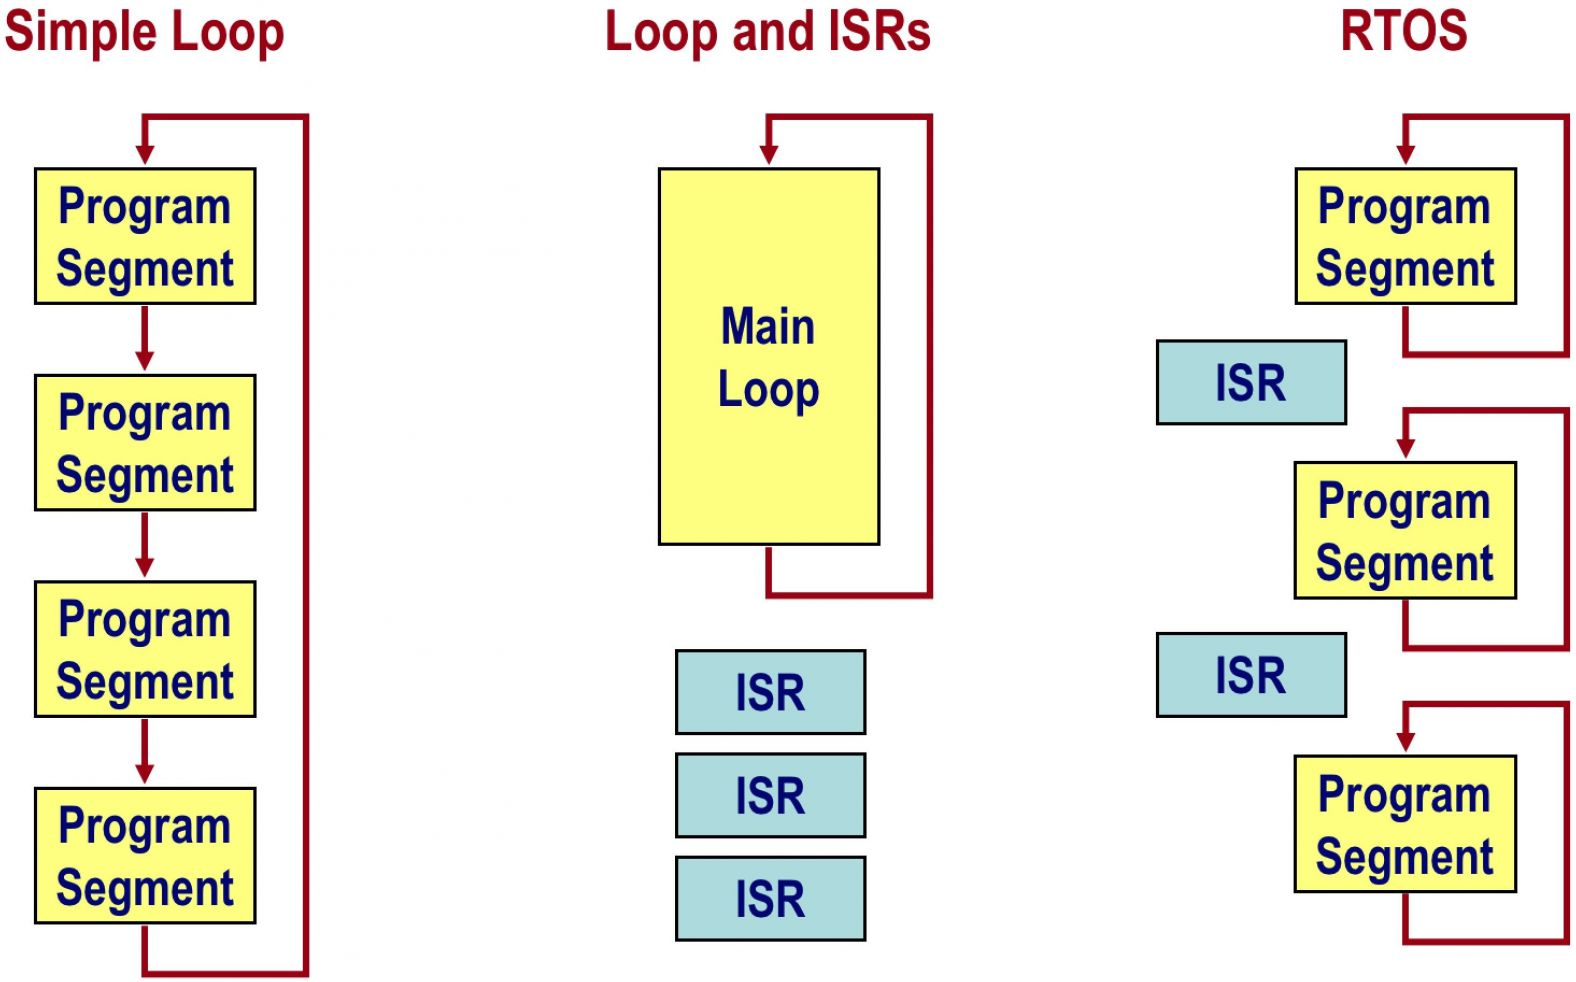
\includegraphics[width=0.3\textwidth]{Pictures/EmbeddedCom/cwrtos2f5c.jpg}
	\caption{Übersicht Programmabläufe}
	\quelle\url{http://www.embedded.com/}
	\label{fig:Programmablauf}
\end{figure}

\begin{table*}
	\begin{tabular}{|l|l|}
		\hline
		\textbf{Beispiel} & \textbf{Echtzeit Typ} \\
		\hline
		Tastatur Controller & Soft Realtime \\
		\hline
		Echtzeit Media Streaming  & Soft Realtime \\
		\hline
		Controller CD Laufwerk  & Hard Realtime \\
		\hline
		Airbag System  & Hard Realtime\\
		\hline
	\end{tabular}
	\caption{Beispiele Echzeitsystem}
	\label{tab:BeispieleEchzeitsystem}
\end{table*}




%Echtzeitbetriebssysteme kommen zum Einsatz wenn neben den oben genannten Anforderungen an ein normales Betriebssystem weitere Anforderungen gestellt werden, die ein normales Betriebssystem nicht berücksichtigt. Dies können beispielsweise garantiert berechenbare Reaktionszeiten sein wie sie in der Fabrikation oder im Automobilbereich gefordert werden oder geringe Leistungsaufnahmen wie bei Komponenten des Internet of Things (IoT). Insgesamt wird zwischen Harten und Weichen Echtzeitkriterien unterschieden. Diese Gliedern sich wie folgt:\newline
%Aufgrund der Eingangs geschilderten Einsatzbereiche ist leich zu erkennen, dass Echzeitbetriebssysteme häufigin Umgebungen zum Einsatz kommen, in denen besondere Anforderungen an die Hardware gestellt werden. Häufig verfügt die Hardware nur über begrenzte Speicherkapazitäten, über geringe Wärmeableitfähigkeiten und damit geringe Rechenleistung. Die zur Verfügung stehende Energie muss bei der Entwicklung ebenfalls berücksichtigt werden. 
%Vor diesem Hintergrund benötigen Echtzeitbetriebssysteme nur wenig Speicherplatz und implementieren Funktionen um den Prozessor und die angeschlossene Peripherie nur kurzzeitig zu belasten und in der restlichen Zeit in den Ruhezustand zu verseten.

\section{FreeRTOS} 
\subsection{Geschichte}
WIP: Christoph
\subsection{Zielsysteme STM32F4 (ARM Cortex M3)}
32 bit Prozessor - Funktionsübersicht, Hinweis Port Teil von FreeRTOS
\subsection{Entwicklungsumgebung}
FreeRTOS ist im Prinzip nicht an eine spezielle Entwicklungsumgebung gebunden. Bevor eine Entwicklung be\-ginnt ist es dennoch ratsam sich einen Überblick über die ver\-fügbaren IDEs\footnote{Integrated Development Environment} zu machen. Der wichtigste Punkt der hier zu nennen ist, ist das Debugging. Da ein Echtzeitbetriebssystem eine weitere Abstraktionsebene hinzufügt und wie eine Art Middleware fungiert, lassen Sich viele RTOS spezifische Funktionen und Eigenschaften wie Queues, Task Stacks etc. nur mühsam mit einem Debugger wie GDB oder OpenOCD untersuchen. Viele der marktgängigen Entwicklungsumgebungen bieten daher spezielle RTOS aware Pakete, so dass ein einfacherer Zugriff auf RTOS Objekte und Eigenschaften möglich ist. Wie die RTOS awareness beim Debugging eingesetzt wird und welche Funktionalitäten sie einem Entwickler bietet wird in Abschnitt \ref{sec:Debugging von Echtzeitsystemen} aufgezeigt. Ein weiterer Punkt der bei der Auswahl der IDE getroffen werden muss sind die Kosten. Bei Propritäre IDEs können oft mehrere tausend Euro Lizenzkosten anfallen, bieten aber den Vorteil der nahtlosen Einbindungen von $\mu$Prozessoren und Echtzeitbetriebssystem (RTOS awareness). Bei der Entwicklung von ARM uProzessoren sind hier Keil (Arm), IAR Workbench und True Studio (Atollic) zu nennen. Diese Entwicklungsumgebungen lassen sich zum Teil auch frei verwenden, allerdings mit starken Einschränkungen wie z.B. maximal Codesize. Auf der nicht proprietären Seiten steht Eclipse CDT zur Verfügung, es ist komplett frei in der Verwendung und hat keine Beschränkungen. Nachteil ist hier, dass die Integration nicht so einfach ist wie bei den proprietären IDEs. RTOS awarness wird bei Eclipse durch die Installation weiterer Plugins erreicht. Ein weiterer Nachteil ist, dass es keine Beispielprojekte für Eclipse CDT und FreeRTOS zur Ver\-fü\-gung stehen, daher müssen Projekte von Grund auf selbst konfiguriert und installiert werden. Da im Laufe dieser Arbeit Eclipse CDT für alle Beispiele verwendet wird, wird in Abschnitt \ref{sec:Einrichtung und Konfiguration} das Aufsetzen einer Basiskonfiguration erklärt. 

\subsection{Einrichten und Konfiguration}
\label{sec:Einrichtung und Konfiguration}
WIP: Eclipse CTD, RTOS AwareNess , Debugger, FileStructure
\begin{itemize}
	\item https://eclipse.org/cdt/
	\item https://launchpad.net/gcc-arm-embedded
\item http://gnuarmeclipse.github.io/plugins/download/
\item http://gnuarmeclipse.github.io/windows-build-tools/
\item http://gnuarmeclipse.github.io/debug/jlink/
\item http://gnuarmeclipse.github.io/debug/openocd/
\item http://freescale.com/lgfiles/updates/Eclipse/KDS
\item Thread Aware 
\item Beispiel Projekt
\item STM32 Cube MX
\item FreeRTOS.org
\end{itemize}

\subsection{Memory Allocation}
Beim Erzeugen von RTOS Objekten wie Tasks, Queues oder Semaphore wird Speicher im RAM benötigt. Für die dynamische Speicherverwaltung wird in C und C++ ge\-wöhnlich die Standard C Funktionen \verb|malloc()| und \verb|free()| verwendet. Die Funktion \verb|malloc()| dient zur Allozierung von freiem Speicher und \verb|free()| zur Freigabe von alloziertem Speicher. Für Echtzeitsysteme die auf einem RTOS aufsetzen, sind diese Funktionen aufgrund der folgende Eigenschaften\cite{MasteringFreeRTOS} ungeeignet\footnote{Heap3 stellt hier eine Ausnahme dar}:
\begin{itemize}
	\item nicht thread safe
	\item nicht deterministisch
	\item tendieren zur Fragmentierung des RAM
	\item schwer zu debuggen
	\item Bibliotheksfunktionen benötigen viel Speicher
\end{itemize}
Des Weiteren sind für einige Einsatzgebiete von embedded Anwendungen Zertifikate erforderlich. Speziell in sicherheitskritischen Anwendungen (medical, military) ist die dynamische Speicherverwaltung als eine potentielle Fehlerquelle auszuschließen. Für einen solchen Fall bietet FreeRTOS ab Version 9.0 die Möglichkeit der statischen Speicherallozierung, diese werden wir am Ende dieses Abschnitts betrachten. In FreeRTOS werden  \verb|malloc()| und \verb|free()| durch die Funktionen  
\begin{lstlisting}[label=lst:vPortMallocFree, numbers = none]
void *pvPortMalloc( size_t xSize );
und
void vPortFree( void *pv );
\end{lstlisting}
ersetzt. Dies hat den Vorteil, dass die Implementierung dieser Funktionen an die jeweilige Anwendung angepasst werden kann. Grundsätzlich bietet FreeRTOS fünf unterschiedliche Beispiel Implementierungen (Heap1 bis Heap5), siehe Abbildung \ref{fig:HeapsEclipse}. 
\begin{figure}[htb!]
	\centering
		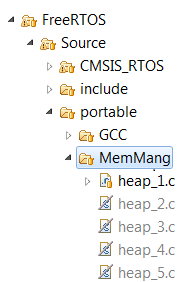
\includegraphics[width=0.2\textwidth]{Pictures/Eclipse/Heaps.png}
	\caption{Einbindung von Heap1. Heap2 bis Heap5 sind vom Build ausgeschlossen}
	\label{fig:HeapsEclipse}
\end{figure}   
Diese stellen prinzipiell schon die ge\-läu\-figsten Implementierungen zur Speicherverwaltung. Es bleibt aber auch weiterhin die Möglichkeit seine eigene Speicherverwaltung zu implementieren. In dieser Arbeit werden wir Heap1 etwas tiefer betrachten um ein grund\-sätz\-liches Verständnis für die FreeRTOS Speicherverwaltung zu bekommen. Heap2 - Heap 5 werden nur kurz beschrieben und können im Detail in \cite{MasteringFreeRTOS}\cite{FreeRTOSAdvanced} nachgelesen werden.      
Wie schon am Anfang dieses Abschnitts beschrieben, werden für alle RTOS Objekte Speicher benötigt, der Speicher für Objekte wie Semaphore und Tasks wird automatisch in den Erzeugerfunktionen alloziert, in dem intern die Funktion \textit{pvPortMalloc()} aufgerufen wird. Die Funktion \verb|xTaskCreate()| dient zum Erzeugen einer FreeRTOS Task. Listing \ref{lst:xTaskCreate} zeigt wie \verb|xTaskCreate()| die Funktion \verb|pvPortMalloc()| verwendet (Zeile 5, 11) um Speicher für den Stack und den Task Control Block zu allozieren.
\begin{lstlisting}[caption={xTaskCreate() memory allocation. Aus Task.c}, linewidth=8cm,captionpos=b, label=lst:xTaskCreate, float=hbt]
StackType_t *pxStack;
/* Allocate space for the stack 
used by the task being created. */
pxStack = 
( StackType_t * ) pvPortMalloc(( ( ( size_t ) usStackDepth ) 
* sizeof( StackType_t ) ) );

if( pxStack != NULL )
{
	/* Allocate space for the TCB. */
	pxNewTCB = ( TCB_t * ) pvPortMalloc( sizeof( TCB_t ) );

	if( pxNewTCB != NULL )
	{
		/* Store the stack location in the TCB. */
		pxNewTCB->pxStack = pxStack;
	}
//...
}

\end{lstlisting}
Alle Objekte die mittels pvPortMalloc() alloziert werden, darunter auch der Kernel selbst, teilen sich einen gemeinsamen Adressraum, siehe Abbildung \ref{fig:AddressSpace}. Eine Speicherzugriffsverletzung ist somit durchaus möglich. In Abschnitt \ref{sec:Memory Protection} wird gezeigt welche Möglichkeit der STM32F4 und FreeRTOS bieten um Speicherzugriffe sicherer zu gestalten.    
\begin{figure}[htb!]
	\centering
		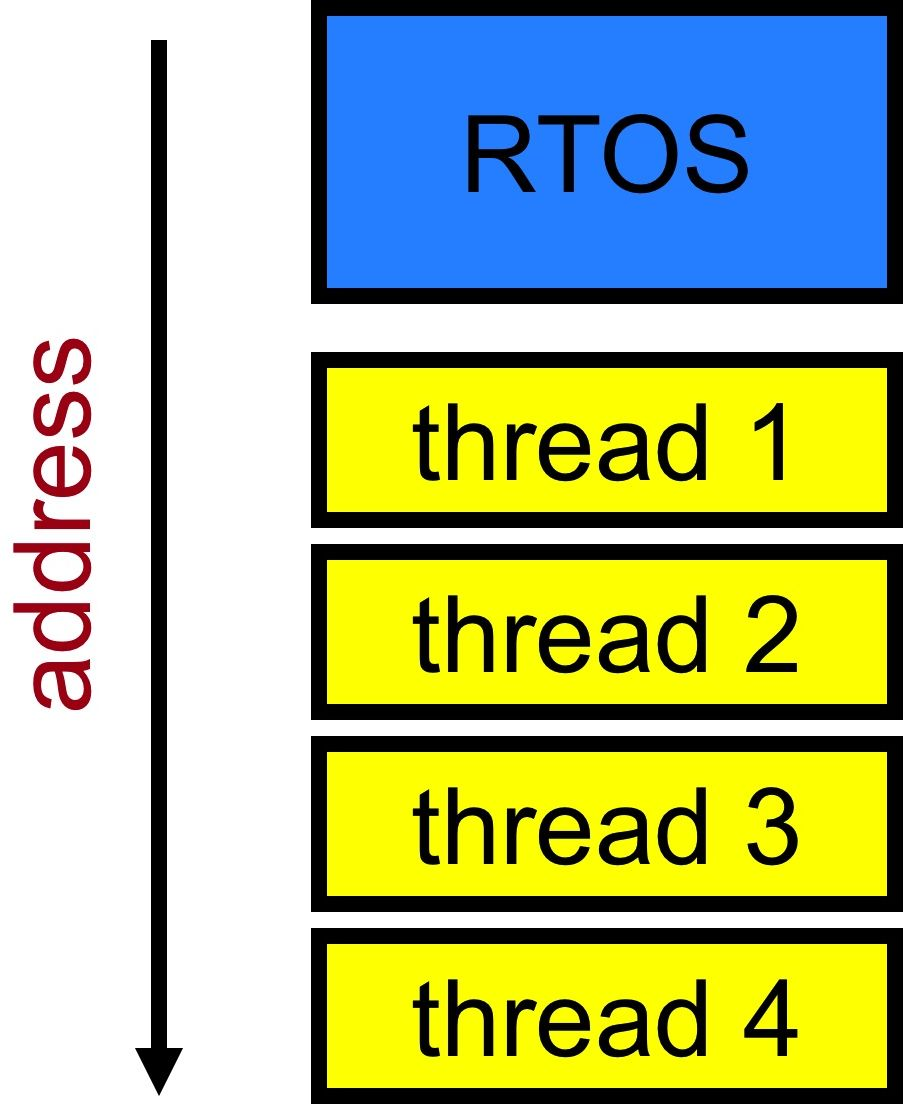
\includegraphics[width=0.2\textwidth]{Pictures/EmbeddedCom/addressSpace.jpg}
	\caption{Adressraum FreeRTOS und Tasks}
	\quelle{Colin Walls - Embedded.com}
	\label{fig:AddressSpace}
\end{figure}    
\subsubsection{FreeRTOS Heap Implementierungen}
Bevor Objekte erzeugt werden können, muss ein Pool an Speicher für die Objekte definiert werden. Die einfachste Form einen Memory Pool zu erzeugen ist ein Array. In FreeRTOS nennt sich dieses Array ucHeap. 
\begin{lstlisting}[label=lst:ucHeap, float=hbt, numbers = none]
static uint8_t ucHeap[ configTOTAL_HEAP_SIZE ];
\end{lstlisting}
\newline
Die Größe des Heaps wird durch das Präprozessor-Define \verb|configTOTAL_HEAP_SIZE | konfiguriert. Die Gesamtgröße berechnet sich wie folgt
\newline
$MaxHeapSize = \verb|configTOTAL_HEAP_SIZE| \ast Wortbreite$. 
\newline
In unserem Fall ist die Wortbreite 32 bit. Heap1 ist sehr einfach, es deklariert lediglich die Funktion pvPortMalloc(). Die Funktion pvPortFree() wird nicht ausimplementiert. Bei vielen embedded Anwendungen wird der Speicher für die benötigten Objekte vor dem Start des Schedulers erzeugt. Eine spätere Freigabe von diesen Resourcen ist nicht nötig, da die Objekte über die gesamte Laufzeit des Programms bestehen sollen. Genau für solche Anwendungen steht Heap1 zur Verfügung. Abbildung \ref{fig:Heap1} zeigt wie sich der Speicher nach dem Erzeugen von zwei Tasks aussieht. Für jede Task wird ein TCB und ein Stack erzeugt, die Speicherobjekte liegen direkt hintereinander, da pvPortFree() nicht implementiert ist, kommt es auch nicht zu einer Fragmentierung des Speichers. Diese lineare Speicherzuweisung gilt für alle Objekte die mittels pvPortMalloc() alloziert werden, dazu gehören sowohl RTOS spezifische Objekte als auch Objekte die durch den Benutzer erzeugt werden. 
\begin{figure}[ht!]
	\centering
		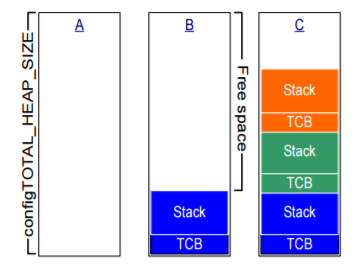
\includegraphics[width=0.3\textwidth]{Pictures/FreeRTOSOrg/heap1Alg.png}
	\caption{Beispiel Speicherbelegung nach drei Instanziierung von Tasks}
	\quelle{FreeRTOS.org}
	\label{fig:Heap1}
\end{figure}
Nachfolgend ein Kurzüberblick über die nicht beschriebenen Beispiel Implementierungen.  
\begin{itemize}
	\item Heap2 - Ähnlich Heap1. Erlaubt Speicherfreigabe. Best Fit Algorithmus zur Speicherallozierung.
	\item Heap3 - Verwendet C Library Malloc() und free() und deaktiviert den Scheduler zur Speicherallozierung.
	\item Heap4 - Ähnlich Heap1 und Heap2. Verwendet First Fit Algorithmus zur Speicherallozierung. Verbindet mehrer kleinere Speicherblöcke in einen großen. Minimiert Speicherfragmentierung
	\item Heap5 - Gleicher Algorithmus wie Heap4 allerdings können mehrere Memory Pools erzeugt werden.
\end{itemize}
\subsubsection{Memory Protection}
\label{sec:Memory Protection}
STM32F4 spezifisch, MPU vorhanden
\begin{figure}[hb!]
	\centering
		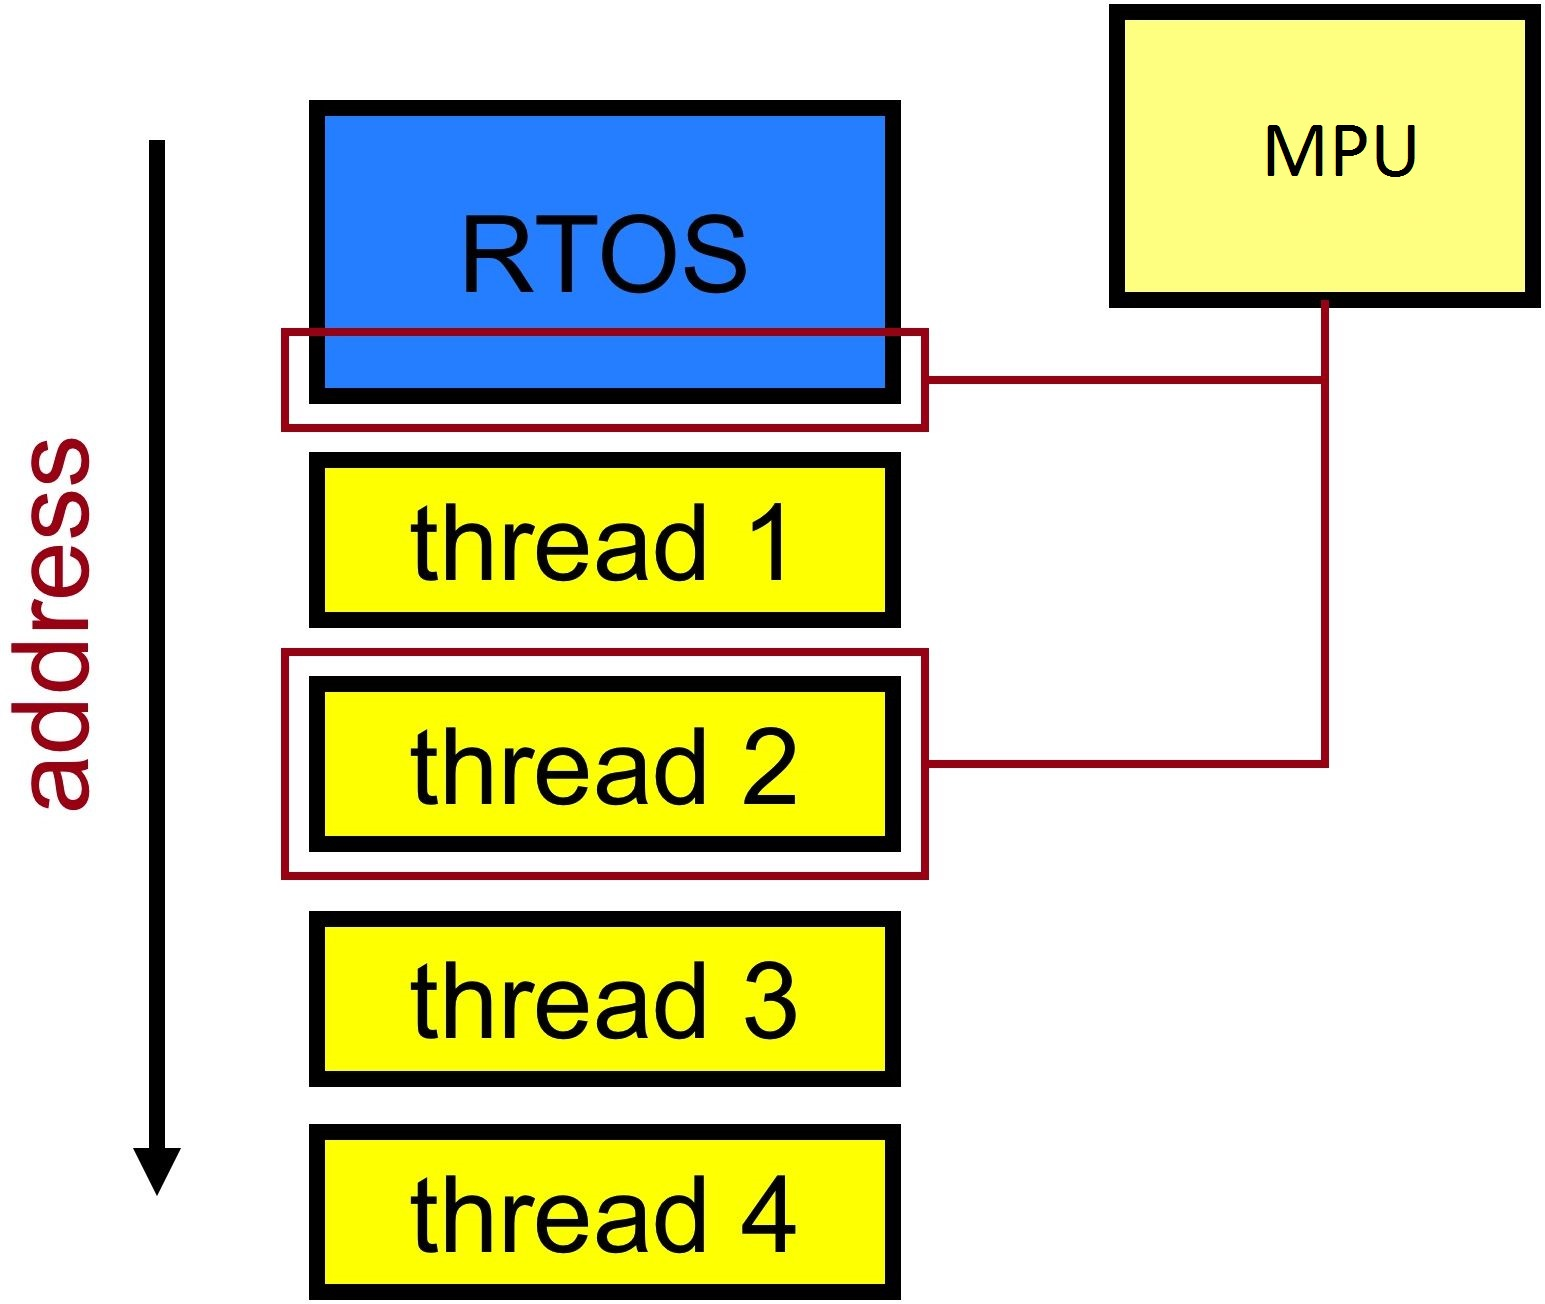
\includegraphics[width=0.3\textwidth]{Pictures/EmbeddedCom/addressSpaceMMU}
	\caption{Adressraum FreeRTOS und Tasks mit Memory Protection}
	\quelle{Colin Walls - Embedded.com}
	\label{fig:AddressSpaceMMU}
\end{figure} 
   
\subsubsection{Static Memory Allocation}
\subsection{Scheduling}
\label{Scheduling}
Blocked - Running :D FSM fertig
\subsection{Intertask Kommunikation}
Queues, Semaphore, Notify, Event Groups
\subsection{Interrupt Handling}
Deamon Task,
\subsection{Low Power Modes auf Stm32F4}
\label{sec:Low Power Modes}
Echtzeitbetriebssysteme kommen immer häufiger in akkubetriebenen embedded Systemen zum Einsatz. Solche Systeme verlangen eine effiziente Nutzung der Energieressourcen um einen möglichst langen Betrieb zu gewährleisten. Bezogen auf den uProzessor gibt es im Prinzip zwei Wege Energie einzusparen:
\begin{itemize}
	\item Heruntertakten des uProzessors.
	\item Das System schlafenlegen, wenn keine weiteren Aufgaben anstehen.
\end{itemize}
Das Heruntertakten des uProzessors ist unabhängig vom Einsatz eines RTOS, daher werden wir hier nur den zweiten Punkt genauer betrachten, das Schlafenlegen des uProzessors. 
\begin{figure}[htb!]
	\centering
		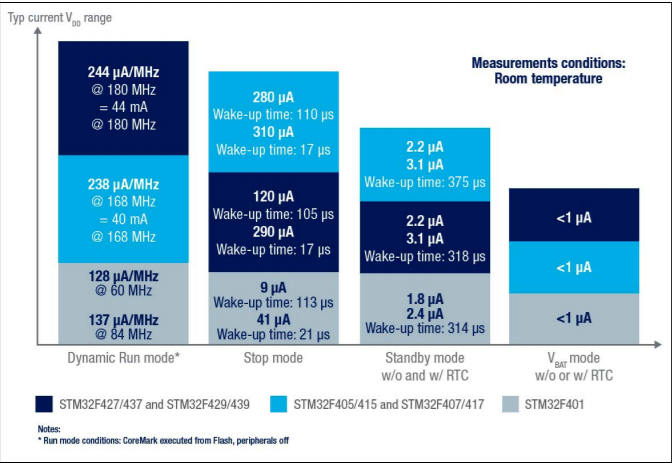
\includegraphics[width=0.4\textwidth]{Pictures/STM32F4/powerConsumption.png}
	\caption{Energieaufnahme für STM32F4 in SleepModes}
	\quelle{STM32F4 - Power Modes}
	\label{fig:powerconsum}
\end{figure}
Abbildung \ref{fig:powerconsum} zeigt wie sich die Stromaufnahme beim STM32F4 von 40mA (@168 MHz) auf 2,2$\mu$A im Tiefschlafmodus reduzieren lässt. 
In einfachen Anwendung ist der Zustand in dem ein Gerät schlafen gehen kann, relativ leicht zu ermitteln. In komplexen Systemen die auf einem Echtzeitbetriebssystem wie FreeRTOS aufsetzen und mehrere Task mög\-li\-cherweise auf unterschiedliche Ressourcen warten, wird es schon schwierig. In diesem Abschnitt wird gezeigt welche Funktionen FreeRTOS zur Ver\-fü\-gung stellt, um einen energieeffizienten Betrieb zu gewährleisten. Eine Mög\-lich\-keit ist die Idle - Hook Funktion. Wie bereits in Abschnitt \ref{Scheduling} beschrieben, wird die IDLE Task von FreeRTOS aktiviert, sobald sich alle User-Tasks im Blocked Zustand befinden. Durch konfigurieren des Präprozessor-Defines        
\begin{lstlisting}[label=lst:defineIdleHook, numbers = none]
#define configUSE_IDLE_HOOK  1; 
\end{lstlisting}
\begin{lstlisting}[caption={Aufruf der IdleTask Hook Funktion. Aus Task.c},captionpos=b, label=lst:xIdleTaskHook, float=htb!]
static portTASK_FUNCTION( prvIdleTask, pvParameters )
{
	/* Stop warnings. */
	( void ) pvParameters;

	/** THIS IS THE RTOS IDLE TASK - WHICH IS CREATED AUTOMATICALLY WHEN THE
	SCHEDULER IS STARTED. **/

	for( ;; )	{
//skipped some code
#if ( configUSE_IDLE_HOOK == 1 )
{
	extern void vApplicationIdleHook( void );
	/* Call the user defined function from within the idle task.  This
	allows the application designer to add background functionality
	without the overhead of a separate task.
	NOTE: vApplicationIdleHook() MUST NOT, UNDER ANY CIRCUMSTANCES,
	CALL A FUNCTION THAT MIGHT BLOCK. */
	
	vApplicationIdleHook();
}
//guess what.. skipped more code
}     
\end{lstlisting}
kann die Idle-Hook Funktion aktiviert werden. Diese wird immer aufgerufen, sobald die Idle Task in den Zustand Running wechselt. Die Funktionalität der Idle-Hook Funktion kann frei vom Entwickler implementiert werden. Listing \ref{lst:xIdleHookExamp} zeigt Pseudocode zu einer beispielhaften Implementierung der Idle Hook Funktion. Bevor das System schlafen gelegt werden kann müssen alle GPIOS und IRQs konfiguriert werden, so dass das System nicht unnötiger weise aufwacht. Des Weiteren werden alle nicht benötigten GPIOS auf Analog gestellt um Energie zu sparen. Als einzige Interrupt-Quelle wird hier eine externe RTC konfiguriert. Mit dem Aufruf von HAL\_PWR\_EnterSTOPMode() wird der uProzessor in den Schlafmodus versetzt. Die Funktion wird erst wieder verlassen sobald der externe Interrupt der RTC ausgelöst wurde. Danach werden alle GPIOs rekonfiguriert. Ein weiterer Schritt der noch unternommen werden muss, ist das informieren einer User-Task z.B. mittels Notify oder Message, so dass das System nicht beim nächsten Tick Interrupt wieder die Idle Task aktiviert. Nachteil dieser Variante ist, dass die Nutzung von Software Timer nicht mehr möglich ist. FreeRTOS würde die Idle Hook Funktion auch aufrufen und sich schlafen legen, wenn noch Software Timer aktiv sind. Die Nutzung von absoluten Zeiten ist ebenfalls nicht mehr möglich, da nach der Deaktivierung des Tick Interrupts der Tickcount nicht mehr korrekt ist. Abhilfe schafft hier eine weitere Funktionalität die FreeRTOS zur Verfügung stell, den sogenannten Tickless Idle Mode. To be continued ....
\begin{lstlisting}[caption={Beispiel Implementierung der Idle Hook Funktion},captionpos=b, label=lst:xIdleHookExamp, float=hbt!]
extern "C" void vApplicationIdleHook( void ){
	/* Systick Interrupt deaktivieren */
	SysTick->CTRL &= ~SysTick_CTRL_TICKINT_Msk;
	//RTC konfigurieren
	setRTCWakeupTime();
	//externen Interrupt durch RTC aktivieren
	enableRTCInterrupt();
	//deaktiviere alle anderen Interrupt Quellen
	deactivateExternalDevices();
	setAllGPIOsToAnalog(); 
	disableGPIOClocks();
	//MCU stoppen und schlafen ZzZZz
	HAL_PWR_EnterSTOPMode(PWR_LOWPOWERREGULATOR_ON, PWR_STOPENTRY_WFI); 
	//Aufgewacht...the show must go on
	//aktiviere Systick
	SysTick->CTRL |= SysTick_CTRL_TICKINT_Msk;
	//reaktiviere GPIO Clocks
	enableGPIOClocks();
	//reaktiviere Externe Interrupt Quellen
	enableExternalInterrupts();	
}
\end{lstlisting}
\subsection{FreeRTOS in der Praxis - Ein real System}
Ad-hoc System? 
\section{Komplexität durch Nebenläufigkeit}
Probleme die bei der Entwicklung auftreten, Häufige Bugs, Speicherüberlauf (Stacktools)
\section{Debugging von Echtzeitsystemen}
TracerLyzer, RtosAwarenes, ThreadAwareness, Hardware Debugging Probes 
\label{sec:Debugging von Echtzeitsystemen}
\section{Echtzeitanalyse}
Uff :)
\label{sec:Echtzeitanalyse} 

 
\section{Zusammenfassung}
\pagebreak
\bibliographystyle{abbrv}
\bibliography{literatur} % Daten aus der Datei literatur.bib verwenden.
\end{document}

